\clearpage
\subsection{Graphical Applications with SwinGame} % (fold)
\label{sub:graphical_applications_with_swingame}

SwinGame is a 2D game creation library. It contains a number of resources that you can use to create small games using the C programming language. To get started with SwinGame you need to download a \emph{template} from the website. The template includes everything you need to get started creating a game in SwinGame.

\subsubsection{Installing SwinGame} % (fold)
\label{ssub:installing_swingame}

The good news is that SwinGame does not require you to install anything on Mac OS or Windows. On Linux you will need to install some libraries, and compile the SwinGame library. The instructions for this are on the SwinGame web site: \url{http://www.swingame.com/wiki/index.php/SwinGame_3_Beta}.

The SwinGame templates contain an already started project template. This includes the SwinGame library, scripts to build your program, and some basic resources (images, sounds, fonts) used in the SwinGame splash screen.

\begin{figure}[h]
   \centering
   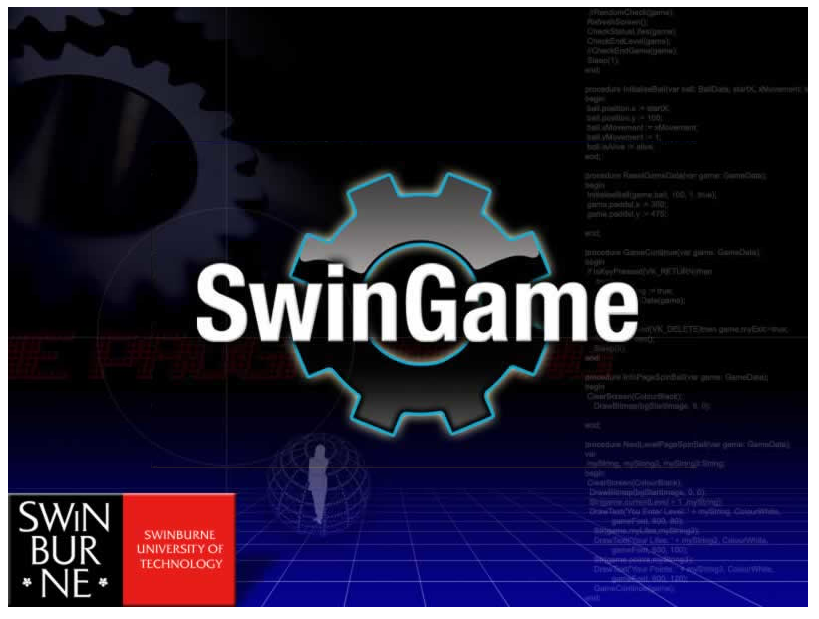
\includegraphics[width=0.5\textwidth]{./topics/programs-and-compilers/images/SwinGameSplash} 
   \caption{SwinGame splash screen}
   \label{fig:swingame-splash}
\end{figure}

\begin{figure}[h]
   \centering
   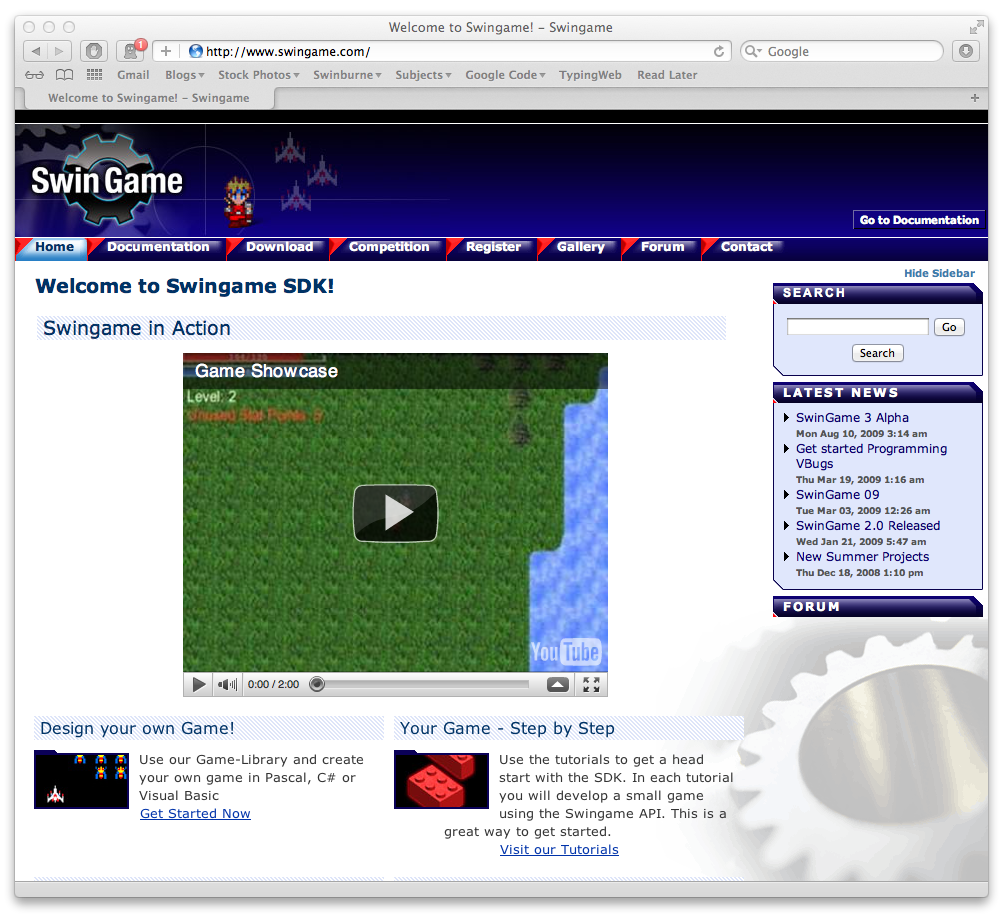
\includegraphics[width=0.5\textwidth]{./topics/programs-and-compilers/images/SwinGameSite} 
   \caption{SwinGame website}
   \label{fig:swingame-site}
\end{figure}


% subsubsection installing_swingame (end)

\clearpage
\subsubsection{Coding a SwinGame} % (fold)
\label{ssub:coding_a_swingame}

The SwinGame project template contains a number of directories to organise your projects code and resources. Within the project directory itself you will find the following files and directories:

\begin{itemize}
  \item \textbf{bin}: When you compile your game it will be placed into this directory. The name \emph{bin} indicates that this contains the \emph{binary} version of the program, the one that contains the \nameref{sub:machine_code}.
  \item \textbf{build.sh}: This file contains a Bash script that will compile your project for you. When you run this script it will compile the code in the \emph{src} directory, and place the resulting game with its resources in the \emph{bin} directory.
  \item \textbf{lib}: Contains the libraries used by SwinGame. This includes the C code used to access these libraries which you can browse if you are interested in seeing what code is available to you.
  \item \textbf{Resources}: This directory contains the resources used by your game. This includes images, sounds, fonts, and other resources. When you want to use your own resources they will need to be placed under this directory in the appropriate subdirectory.
  \item \textbf{src}: Is the directory that will contain your game's code. The standard template contains a basic template you can use to get started.
  \item \textbf{tmp}: Stores temporary files created by the compiler. 
\end{itemize}

To start experimenting with SwinGame, you should download a new project and compile it. The following steps outline how to do this:
\begin{enumerate}
  \item \textbf{Download} the \textbf{gcc} version of SwinGame for your Operating System (You can download this from \url{http://www.swingame.com/wiki/index.php/SwinGame_3_Beta}). 
  \item \textbf{Extract} the \emph{Project Template} from the file you downloaded.
  \item \textbf{Rename} the directory to the name of your game, call the first one \textbf{HelloWorld}.
  \item \textbf{Open} a \nameref{sub:terminal}, and \emph{change directory} so that you are in your game directory, inside the \emph{HelloWorld} directory, if that is what you called your game.
  \item \textbf{Run} the \emph{build.sh} script. You do this by typing \texttt{./build.sh} and pressing enter.
  \item \textbf{Run} your game using the following, where \texttt{HelloWorld} can be replaced with the name you used for the game:
  \begin{itemize}
    \item \textbf{Linux}: \texttt{./bin/Release/HelloWorld}
    \item \textbf{Mac OS}: \texttt{./bin/Release/HelloWorld.app/Contents/MacOS/HelloWorld}
    \item \textbf{Windows}: \texttt{./bin/Release/HelloWorld.exe}
  \end{itemize}
\end{enumerate}

Once you have this compiling and running you can start to play with the source code. The code for your SwinGame can be found in the \textbf{\texttt{src}} folder. This includes a \texttt{\textbf{main.c}} file, where you can place your source code.

% subsubsection coding_a_swingame (end)

% subsection graphical_applications_with_swingame (end)